% Options for packages loaded elsewhere
\PassOptionsToPackage{unicode}{hyperref}
\PassOptionsToPackage{hyphens}{url}
%
\documentclass[
]{book}
\usepackage{lmodern}
\usepackage{amssymb,amsmath}
\usepackage{ifxetex,ifluatex}
\ifnum 0\ifxetex 1\fi\ifluatex 1\fi=0 % if pdftex
  \usepackage[T1]{fontenc}
  \usepackage[utf8]{inputenc}
  \usepackage{textcomp} % provide euro and other symbols
\else % if luatex or xetex
  \usepackage{unicode-math}
  \defaultfontfeatures{Scale=MatchLowercase}
  \defaultfontfeatures[\rmfamily]{Ligatures=TeX,Scale=1}
\fi
% Use upquote if available, for straight quotes in verbatim environments
\IfFileExists{upquote.sty}{\usepackage{upquote}}{}
\IfFileExists{microtype.sty}{% use microtype if available
  \usepackage[]{microtype}
  \UseMicrotypeSet[protrusion]{basicmath} % disable protrusion for tt fonts
}{}
\makeatletter
\@ifundefined{KOMAClassName}{% if non-KOMA class
  \IfFileExists{parskip.sty}{%
    \usepackage{parskip}
  }{% else
    \setlength{\parindent}{0pt}
    \setlength{\parskip}{6pt plus 2pt minus 1pt}}
}{% if KOMA class
  \KOMAoptions{parskip=half}}
\makeatother
\usepackage{xcolor}
\IfFileExists{xurl.sty}{\usepackage{xurl}}{} % add URL line breaks if available
\IfFileExists{bookmark.sty}{\usepackage{bookmark}}{\usepackage{hyperref}}
\hypersetup{
  pdftitle={Machine Learning for Social Scientists},
  pdfauthor={Jorge Cimentada},
  hidelinks,
  pdfcreator={LaTeX via pandoc}}
\urlstyle{same} % disable monospaced font for URLs
\usepackage{color}
\usepackage{fancyvrb}
\newcommand{\VerbBar}{|}
\newcommand{\VERB}{\Verb[commandchars=\\\{\}]}
\DefineVerbatimEnvironment{Highlighting}{Verbatim}{commandchars=\\\{\}}
% Add ',fontsize=\small' for more characters per line
\usepackage{framed}
\definecolor{shadecolor}{RGB}{248,248,248}
\newenvironment{Shaded}{\begin{snugshade}}{\end{snugshade}}
\newcommand{\AlertTok}[1]{\textcolor[rgb]{0.94,0.16,0.16}{#1}}
\newcommand{\AnnotationTok}[1]{\textcolor[rgb]{0.56,0.35,0.01}{\textbf{\textit{#1}}}}
\newcommand{\AttributeTok}[1]{\textcolor[rgb]{0.77,0.63,0.00}{#1}}
\newcommand{\BaseNTok}[1]{\textcolor[rgb]{0.00,0.00,0.81}{#1}}
\newcommand{\BuiltInTok}[1]{#1}
\newcommand{\CharTok}[1]{\textcolor[rgb]{0.31,0.60,0.02}{#1}}
\newcommand{\CommentTok}[1]{\textcolor[rgb]{0.56,0.35,0.01}{\textit{#1}}}
\newcommand{\CommentVarTok}[1]{\textcolor[rgb]{0.56,0.35,0.01}{\textbf{\textit{#1}}}}
\newcommand{\ConstantTok}[1]{\textcolor[rgb]{0.00,0.00,0.00}{#1}}
\newcommand{\ControlFlowTok}[1]{\textcolor[rgb]{0.13,0.29,0.53}{\textbf{#1}}}
\newcommand{\DataTypeTok}[1]{\textcolor[rgb]{0.13,0.29,0.53}{#1}}
\newcommand{\DecValTok}[1]{\textcolor[rgb]{0.00,0.00,0.81}{#1}}
\newcommand{\DocumentationTok}[1]{\textcolor[rgb]{0.56,0.35,0.01}{\textbf{\textit{#1}}}}
\newcommand{\ErrorTok}[1]{\textcolor[rgb]{0.64,0.00,0.00}{\textbf{#1}}}
\newcommand{\ExtensionTok}[1]{#1}
\newcommand{\FloatTok}[1]{\textcolor[rgb]{0.00,0.00,0.81}{#1}}
\newcommand{\FunctionTok}[1]{\textcolor[rgb]{0.00,0.00,0.00}{#1}}
\newcommand{\ImportTok}[1]{#1}
\newcommand{\InformationTok}[1]{\textcolor[rgb]{0.56,0.35,0.01}{\textbf{\textit{#1}}}}
\newcommand{\KeywordTok}[1]{\textcolor[rgb]{0.13,0.29,0.53}{\textbf{#1}}}
\newcommand{\NormalTok}[1]{#1}
\newcommand{\OperatorTok}[1]{\textcolor[rgb]{0.81,0.36,0.00}{\textbf{#1}}}
\newcommand{\OtherTok}[1]{\textcolor[rgb]{0.56,0.35,0.01}{#1}}
\newcommand{\PreprocessorTok}[1]{\textcolor[rgb]{0.56,0.35,0.01}{\textit{#1}}}
\newcommand{\RegionMarkerTok}[1]{#1}
\newcommand{\SpecialCharTok}[1]{\textcolor[rgb]{0.00,0.00,0.00}{#1}}
\newcommand{\SpecialStringTok}[1]{\textcolor[rgb]{0.31,0.60,0.02}{#1}}
\newcommand{\StringTok}[1]{\textcolor[rgb]{0.31,0.60,0.02}{#1}}
\newcommand{\VariableTok}[1]{\textcolor[rgb]{0.00,0.00,0.00}{#1}}
\newcommand{\VerbatimStringTok}[1]{\textcolor[rgb]{0.31,0.60,0.02}{#1}}
\newcommand{\WarningTok}[1]{\textcolor[rgb]{0.56,0.35,0.01}{\textbf{\textit{#1}}}}
\usepackage{longtable,booktabs}
% Correct order of tables after \paragraph or \subparagraph
\usepackage{etoolbox}
\makeatletter
\patchcmd\longtable{\par}{\if@noskipsec\mbox{}\fi\par}{}{}
\makeatother
% Allow footnotes in longtable head/foot
\IfFileExists{footnotehyper.sty}{\usepackage{footnotehyper}}{\usepackage{footnote}}
\makesavenoteenv{longtable}
\usepackage{graphicx,grffile}
\makeatletter
\def\maxwidth{\ifdim\Gin@nat@width>\linewidth\linewidth\else\Gin@nat@width\fi}
\def\maxheight{\ifdim\Gin@nat@height>\textheight\textheight\else\Gin@nat@height\fi}
\makeatother
% Scale images if necessary, so that they will not overflow the page
% margins by default, and it is still possible to overwrite the defaults
% using explicit options in \includegraphics[width, height, ...]{}
\setkeys{Gin}{width=\maxwidth,height=\maxheight,keepaspectratio}
% Set default figure placement to htbp
\makeatletter
\def\fps@figure{htbp}
\makeatother
\setlength{\emergencystretch}{3em} % prevent overfull lines
\providecommand{\tightlist}{%
  \setlength{\itemsep}{0pt}\setlength{\parskip}{0pt}}
\setcounter{secnumdepth}{5}
\usepackage{booktabs}
\usepackage[]{natbib}
\bibliographystyle{apalike}

\title{Machine Learning for Social Scientists}
\author{Jorge Cimentada}
\date{2020-03-02}

\begin{document}
\frontmatter
\maketitle

{
\setcounter{tocdepth}{1}
\tableofcontents
}
\mainmatter
\hypertarget{preface}{%
\chapter*{Preface}\label{preface}}
\addcontentsline{toc}{chapter}{Preface}

Notes, content and exercises for the RECSM 2020 course Machine Learning for Social Scientists. These are intended to introduce social scientists to concepts in machine learning using traditional social science examples and datasets. Currently, it is not intended to be a book but rather supporting material for the course. Perhaps it evolves enough to be a book some day.

\hypertarget{machine-learning-for-social-scientists}{%
\chapter{Machine Learning for Social Scientists}\label{machine-learning-for-social-scientists}}

Machine Learning practitioners and Social Scientists share many things in common. These shared traits are mostly related to the transformation, analysis and evaluation of statistical models. In fact, when many of my fellow social scientists take any introductory course on machine learning, I often hear that many of the things they get taught are very common in traditional statistics classes, if not the same. This is good news! This means that you already have a foot inside the field without even knowing it. Machine Learning practitioners use many of the same statistical model we use and also many of transformation techniques that we use. However, there are important differences on how we analyze data and how we answer our questions. In this chapter I will elaborate on how machine learning practitioners have developed strategies different from social scientists for analyzing their data, how their analysis workflow compares to ours and finally, a tour around their way of thinking, which has evolved to be very different from ours.

I hope that by understanding the strategies and techniques that machine learning practitioners use, social scientists would expand their analysis toolbox, allowing us to complement their way of thinking with our strong research design skills and modelling techniques.

\hypertarget{a-different-way-of-thinking}{%
\section{A different way of thinking}\label{a-different-way-of-thinking}}

The first question we want to ask ourselves is, what is machine learning? Machine Learning bears indeed a fancy name which brings to mind thoughts related to artificial intelligence and robots. However, as you'll see throughout the course, most terms and models used in machine learning are actually what we know as \textbf{statistical models}. The overaching difference in the definition of machine learning and social statistics is not the models or new strategies for analyzing data. It is the main objective of the analysis. What is Machine Learning after all?

\begin{quote}
Using statistical methods to learn the data enough to be able to predict it accurately on new data
\end{quote}

That sounds somewhat familiar to us social scientists. Perhaps our goal is not to predict our data but it is certainly to \textbf{learn it} and \textbf{understand it}. In particular, social scientists are interested in figuring out if our theoretical description of the problem fits the data we have collected it. We do that by carefully build a model that explains the problem, we try to learn it really well and finally understand it enough such that if we collected the exact same data again, our explanation would replicate. How does this differ from the way of thinking of machine learning practitioners? The main objective in a machine learning problem is accurate predictions; that is, regardless of how well we understand a problem, we want learn the data well enough to predict it well. Prediction problems are usually concerned with \textbf{building and tweaking} a model that predicts a dependent variable accurately on your data, such that when \textbf{new data} arrives, the model can predict it just as accurately.

The difference between the two cultures (breiman) is the problem of inference versus prediction. That is the fundamental difference between the approach used by social scientists and practitioners of machine learning. However, for having such drastic differences in our objective, we share a lot of common strategies. For example, here's the typical workflow of a social scientist:

\begin{center}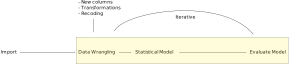
\includegraphics[width=0.99\linewidth]{./img/socsci_wflow1_smaller} \end{center}

This is our safe zone: we understand these steps and we've exercised them many times. We begin by importing our data and inmediately start to clean it. This involves, for example, collapsing fine grained groups into bigger categories, transforming variables using logarithms and creating new variables which reflect important concepts from our theoretical model. Once we're confident with our set of variables, we begin the iterative process of visualizing our data, fitting statistical models and evaluating the fit of the model. This is an iterative process because the results of our model might give us ideas on new variables or how to recode an existing variable. This prompts us to repeat the same process again with the aim of carefully building a model that fits the data well. Well, let me break it to you but this same process is very familiar to the machine learning process:

\begin{center}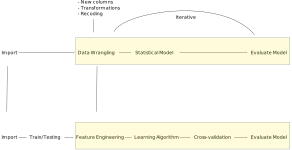
\includegraphics[width=0.99\linewidth]{./img/socsci_wflow3_smaller} \end{center}

They import their data, they wrangle their data, they fit statistical models and they evaluate the fit of their models. They might have different names for the same things but in essence, they are more or less the same. For example, here are some common terms in the machine learning literature which have exact equivalents in social statistics:

\begin{itemize}
\tightlist
\item
  Features --\textgreater{} Variables
\item
  Feature Engineering --\textgreater{} Creating Variables
\item
  Learning Algorithms --\textgreater{} Statistical Models
\item
  Supervised Learning --\textgreater{} Models that have a dependent variable
\item
  Unsupervised Learning --\textgreater{} Models that don't have a dependent variable, such as clustering
\item
  Classifiers --\textgreater{} Models for predicting categorical variables, such as logistic regression
\end{itemize}

and you'll find more around. These are the common steps which you'll find between both fields. However, machine Learning practioners have developed extra steps:

\begin{center}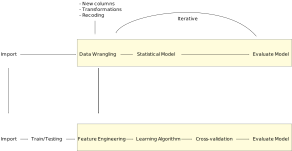
\includegraphics[width=0.99\linewidth]{./img/socsci_wflow4_smaller} \end{center}

\begin{itemize}
\tightlist
\item
  Training/Testing data --\textgreater{} Unknown to us
\item
  Cross-validation --\textgreater{} Unknown to us
\item
  Loss functions --\textgreater{} Model fit --\textgreater{} Known to us but are not predominant (\(RMSE\), \(R^2\), etc\ldots)
\end{itemize}

These are very useful concepts and we'll focus on those in this introduction. In this introduction I won't delve into the statistical models (learning algorithms) used in machine learning these will be discussed in later chapters but I wanted to highlight that although they share similarities with the models used in social statistics, there are many models used in the meachine learning literature which are unknown to us.

\hypertarget{split-your-data-into-trainingtesting}{%
\section{Split your data into training/testing}\label{split-your-data-into-trainingtesting}}

Since the main objective in machine learning is to predict data accurately, all of their strategies are geared toward avoiding overfitting/underfitting. In other words, they want to capture all the signal and ignore the noise:

\begin{Shaded}
\begin{Highlighting}[]
\KeywordTok{library}\NormalTok{(ggplot2)}
\KeywordTok{library}\NormalTok{(patchwork)}
\KeywordTok{library}\NormalTok{(scales)}

\KeywordTok{set.seed}\NormalTok{(}\DecValTok{2313}\NormalTok{)}
\NormalTok{n <-}\StringTok{ }\DecValTok{500}
\NormalTok{x <-}\StringTok{ }\KeywordTok{rnorm}\NormalTok{(n)}
\NormalTok{y <-}\StringTok{ }\NormalTok{x}\OperatorTok{^}\DecValTok{3} \OperatorTok{+}\StringTok{ }\KeywordTok{rnorm}\NormalTok{(n, }\DataTypeTok{sd =} \DecValTok{3}\NormalTok{)}
\NormalTok{age <-}\StringTok{ }\KeywordTok{rescale}\NormalTok{(x, }\DataTypeTok{to =} \KeywordTok{c}\NormalTok{(}\DecValTok{0}\NormalTok{, }\DecValTok{100}\NormalTok{))}
\NormalTok{income <-}\StringTok{ }\KeywordTok{rescale}\NormalTok{(y, }\DataTypeTok{to =} \KeywordTok{c}\NormalTok{(}\DecValTok{0}\NormalTok{, }\DecValTok{5000}\NormalTok{))}

\NormalTok{age_inc <-}\StringTok{ }\KeywordTok{data.frame}\NormalTok{(}\DataTypeTok{age =}\NormalTok{ age, }\DataTypeTok{income =}\NormalTok{ income)}

\NormalTok{y_axis <-}\StringTok{ }\KeywordTok{scale_y_continuous}\NormalTok{(}\DataTypeTok{labels =} \KeywordTok{dollar_format}\NormalTok{(}\DataTypeTok{suffix =} \StringTok{"€"}\NormalTok{, }\DataTypeTok{prefix =} \StringTok{""}\NormalTok{),}
                             \DataTypeTok{limits =} \KeywordTok{c}\NormalTok{(}\DecValTok{0}\NormalTok{, }\DecValTok{5000}\NormalTok{),}
                             \DataTypeTok{name =} \StringTok{"Income"}\NormalTok{)}

\NormalTok{x_axis <-}\StringTok{ }\KeywordTok{scale_x_continuous}\NormalTok{(}\DataTypeTok{name =} \StringTok{"Age"}\NormalTok{)}

\NormalTok{underfit <-}
\StringTok{  }\KeywordTok{ggplot}\NormalTok{(age_inc, }\KeywordTok{aes}\NormalTok{(age, income)) }\OperatorTok{+}
\StringTok{  }\KeywordTok{geom_point}\NormalTok{() }\OperatorTok{+}
\StringTok{  }\KeywordTok{geom_smooth}\NormalTok{(}\DataTypeTok{method =} \StringTok{"lm"}\NormalTok{) }\OperatorTok{+}
\StringTok{  }\NormalTok{y_axis }\OperatorTok{+}
\StringTok{  }\NormalTok{x_axis }\OperatorTok{+}\StringTok{  }
\StringTok{  }\KeywordTok{ggtitle}\NormalTok{(}\StringTok{"Underfit"}\NormalTok{) }\OperatorTok{+}
\StringTok{  }\KeywordTok{theme_linedraw}\NormalTok{()}

\NormalTok{overfit <-}
\StringTok{  }\KeywordTok{ggplot}\NormalTok{(age_inc, }\KeywordTok{aes}\NormalTok{(age, income)) }\OperatorTok{+}
\StringTok{  }\KeywordTok{geom_point}\NormalTok{() }\OperatorTok{+}
\StringTok{  }\KeywordTok{geom_smooth}\NormalTok{(}\DataTypeTok{method =} \StringTok{"loess"}\NormalTok{, }\DataTypeTok{span =} \FloatTok{0.015}\NormalTok{) }\OperatorTok{+}
\StringTok{  }\NormalTok{y_axis }\OperatorTok{+}
\StringTok{  }\NormalTok{x_axis }\OperatorTok{+}\StringTok{  }
\StringTok{  }\KeywordTok{ggtitle}\NormalTok{(}\StringTok{"Overfit"}\NormalTok{) }\OperatorTok{+}
\StringTok{  }\KeywordTok{theme_linedraw}\NormalTok{()}

\NormalTok{goodfit <-}
\StringTok{  }\KeywordTok{ggplot}\NormalTok{(age_inc, }\KeywordTok{aes}\NormalTok{(age, income)) }\OperatorTok{+}
\StringTok{  }\KeywordTok{geom_point}\NormalTok{() }\OperatorTok{+}
\StringTok{  }\KeywordTok{geom_smooth}\NormalTok{(}\DataTypeTok{method =} \StringTok{"loess"}\NormalTok{, }\DataTypeTok{span =} \FloatTok{0.9}\NormalTok{) }\OperatorTok{+}
\StringTok{  }\NormalTok{y_axis }\OperatorTok{+}
\StringTok{  }\NormalTok{x_axis }\OperatorTok{+}\StringTok{  }
\StringTok{  }\KeywordTok{ggtitle}\NormalTok{(}\StringTok{"Ideal fit"}\NormalTok{) }\OperatorTok{+}
\StringTok{  }\KeywordTok{theme_linedraw}\NormalTok{()}

\NormalTok{underfit }\OperatorTok{+}\StringTok{ }\NormalTok{overfit }\OperatorTok{+}\StringTok{ }\NormalTok{goodfit}
\end{Highlighting}
\end{Shaded}

\begin{center}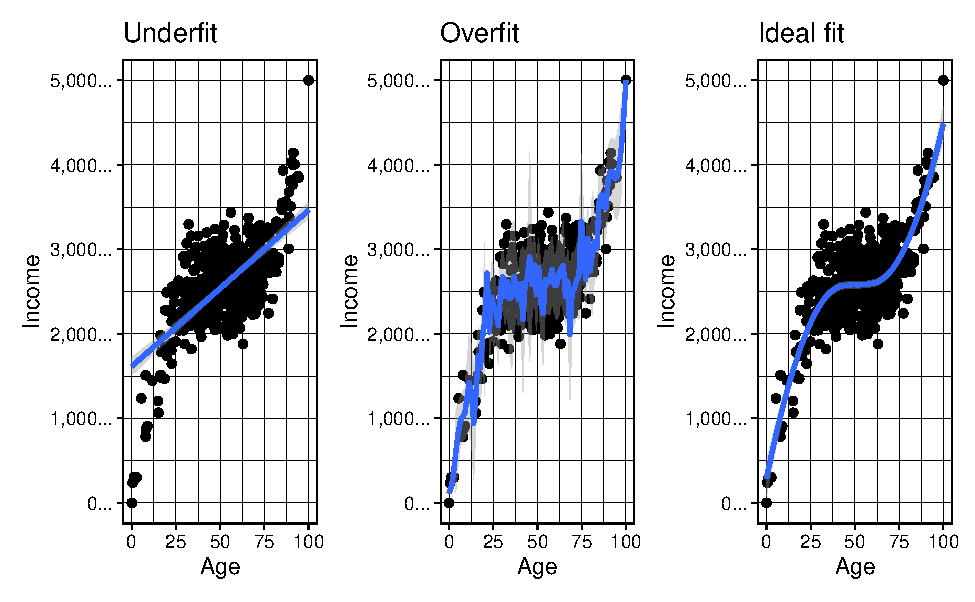
\includegraphics[width=0.99\linewidth]{./figs/unnamed-chunk-4-1} \end{center}

The first plot shows a model which is not flexible, as it fits a straight line without capturing the subtle non-linearities of the data. The second plot is \textbf{too} flexible as it captures much of the random noise of the non-linear relationship. Finally, the third plot shows the ideal fit, where the fitted line is flexible enough to capture the non-linear relationship in the data yet it it is mainly unaffected by the random noise in the data. How would social scientists fit a model? They would take the entire data

\begin{center}\includegraphics[width=0.4\linewidth]{./img/raw_data_wnote} \end{center}

and fit the model on it. How do you know you're overfitting? Is there a metric? Is there a method? Well, one very easy and naive approach is to randomly divide your data into two chunks called training and testing:

\begin{center}\includegraphics[width=0.8\linewidth]{./img/train_testing_df} \end{center}

The training data usually consists of a random sample of around \textasciitilde70\% of the initial data and the testing data a random sample of \textasciitilde30\% of the initial data. If a particular row is in the training data, it \textbf{must not} be on the testing data. If a particular row is in the testing data, it shouldn't be in the training data either. Let me clarify this: being in one chunk should mean that that specific row should \textbf{not} be in the other chunk. These two chunks should be completely independent of each other. Why should splitting the data help us fix the problem of overfitting? Because you can elaborate your model in the training set as much as you want, and when you're confident enough, the testing set can serve as an \textbf{unseen, pristine source of data} on which you can evaluate your model.

In the training chunk

\begin{center}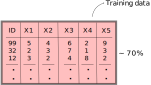
\includegraphics[width=0.5\linewidth]{./img/training_df} \end{center}

fit your model and tweak it enough such that you can evaluate whether it's making accurate predictions. You can think of this chunk as the complete data to perform your analysis. It is the equivalent of the initial data where social scientists fit their data (that is, without partitiong). Once you're very comfortable with your model, the best recipe for checking whether your model was overfit is to use this fitted model to predict on \textbf{the other chunk of data} (the testing data):

\begin{center}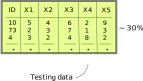
\includegraphics[width=0.5\linewidth]{./img/testing_df} \end{center}

If you tweaked your model in such a way that it learned the noise of your training data, it will perform poorly on the testing data, since you the model didn't capture the overall trend in the data but rather the noise.

For the sake of an example, let's suppose that you fit your model several times on the \textcolor{red}{training} data, tweaking it to improve performance. When you think you're ready, you use this model to predict on the \textcolor{#D4FF2A}{testing} data and find out that the model was indeed overfitting the data. You go back to the \textcolor{red}{training} data, tweak some more, run some models again and when you think you're model is ready again, you predict on your \textcolor{#D4FF2A}{testing} data again and find that it improved. Then you repeate the process again, \(3\), \(4\), \(5\), etc\ldots{} times. If you do that, you will, in very subtle ways, start to \textbf{overfit} your model on the \textcolor{#D4FF2A}{testing} data! Think about it: you're fitting a model N times on your \textcolor{red}{training} data, evaluating its fit on the \textcolor{#D4FF2A}{testing} data and then \textbf{tweaking} again to improve the prediction on the \textcolor{#D4FF2A}{testing} data. The \textcolor{#D4FF2A}{testing} data should serve as the final dataset to compare your model: you should not tweak the model again after seeing how your model fits the \textbf{unseen} \textcolor{#D4FF2A}{testing} data.

How can we evaluate whether we're overfitting with the \textcolor{red}{training} data alone, then? \textbf{Enter cross-validation}

\hypertarget{cross-validation}{%
\section{Cross-validation}\label{cross-validation}}

The idea behind cross-validation is to allow the analyst check whether they're overfitting the data without predicting on the \textcolor{#D4FF2A}{testing} data. How does it work? First, we \textbf{only} select our \textcolor{red}{training} data

\begin{center}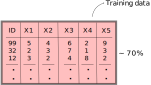
\includegraphics[width=0.5\linewidth]{./img/training_df} \end{center}

and replicate the data 10 times

\begin{center}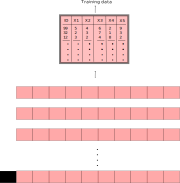
\includegraphics[width=0.95\linewidth]{./img/train_cv2_smaller} \end{center}

The 10 rectangular red rows below the \textcolor{red}{training} data, contain an exact replica of the initial \textcolor{red}{training} data. That is, if the initial \textcolor{red}{training} data has 500 rows and 10 columns, then each of these red rectangle rows also has 500 rows and 10 columns. The idea behind this approach is that you now have 10 different chances of tweaking your model:

\begin{center}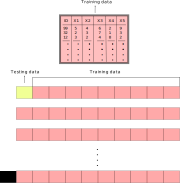
\includegraphics[width=0.95\linewidth]{./img/train_cv3_smaller} \end{center}

and then

\begin{center}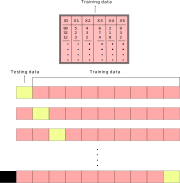
\includegraphics[width=0.95\linewidth]{./img/train_cv4_smaller} \end{center}

This approach offers a way to iterate as many times as you want on tweaking your model and predicting on the cross-validated \textcolor{#D4FF2A}{testing} data without actually predicting on the initial \textcolor{#D4FF2A}{testing} dataset. This is the least bad approach that is currently accepted in the literature. Why is it the least bad approach? Because if we tweak the model on these 10 replicas one time, then a second time, then a third time, etc\ldots, we'll also start overfitting on each of these 10 slots. The superiority of this approach over tweaking on the \textcolor{red}{training} data is that since we have 10 replicas, we can take the average of our model fit and also obtain standard errors. This allows to have a somewhat balanced account of how our model fit is doing and the uncertainty around it.

That said, since we will always overfit in someway using a cross-validation approach, the final error of your model fit on the \textcolor{red}{training} data will always be over optimistic (lower error than what you will actually have, if you predicted on the \textbf{pristine} \textcolor{#D4FF2A}{testing} data.

\hypertarget{regularization}{%
\chapter{Regularization}\label{regularization}}

Regularization is a common topic in machine learning and bayesian statistics. In this document, we will describe the three most common regularized linear models in the machine learning literature and introduce them in the context of the PISA data set. At the end of the document you'll find exercises that will put your knowledge to the test. Most of this material is built upon Boehmke \& Greenwell (2019) and Friedman et al.~(2001).

\hypertarget{ridge-regularization}{%
\section{Ridge regularization}\label{ridge-regularization}}

Do no let others fool you into thinking that ridge regression is a fancy artificial intelligence algorithm. Are you familiar with linear regression? If you are, then ridge regression is just a very \textbf{simple} adaptation of linear regression.

The whole aim of linear regression, or Ordinary Least Squares (OLS), is to minimize the sum of the squared residuals. In other words, fit \texttt{N} number of regression lines to the data and keep only the one that has the lowest sum of squared residuals. In simple formula jargon, OLS tries to \textbf{minimize} this:

\begin{equation}
RSS = \sum_{k = 1}^n(actual_i - predicted_i)^2
\end{equation}

For each fitted regression line, you compare the predicted value (\(predicted_i\)) versus the actual value (\(actual_i\)), square it, and add it all up. Each fitted regression line then has an associated Residual Sum of Squares (RSS) and the linear model chooses the line with the lowest RSS.

\begin{quote}
Note: Social scientists are familiar with the RSS and call it just by it's name. However, be aware that in machine learning jargon, the RSS belongs to a general family called \textbf{loss functions}. Loss functions are metrics that evaluate the \textbf{fit} of your model and there are many around (such as AIC, BIC or R2).
\end{quote}

Ridge regression takes the previous RSS loss function and adds one term:

\begin{equation}
RSS + \lambda \sum_{k = 1}^n \beta^2_j
\end{equation}

The new term is called a \emph{shrinkage penalty} because it forces each coefficient \(\beta_j\) closer to zero by squaring it. The shrinkage part is clearer once you think of this term as forcing each coefficient to be as small as possible but also considering having the smallest Residual Sum of Squares (RSS). In other words, we want the smallest coefficients that don't affect the fit of the line (RSS).

An intuitive example is to think of RSS and \(\sum_{k = 1}^n \beta^2_j\) as two separate things. RSS estimates how the model fits the data and \(\sum_{k = 1}^n \beta^2_j\) limits how much you overfit the data. Finally, the little \(\lambda\) between these two terms can be interpreted as a ``weight''. The higher the lambda, the higher the weight that will be given to the shrinkage term of the equation. If \(\lambda\) is 0, then multiplying 0 by \(\sum_{k = 1}^n \beta^2_j\) will always return zero, forcing our previous equation to simply be reduced to the single term \(RSS\).

Why is there a need to ``limit'' how well the model fits the data? Because we, social scientists and data scientists, very commonly \textbf{overfit} the data. The plot below shows a simulation from \href{https://drsimonj.svbtle.com/ridge-regression-with-glmnet}{Simon Jackson} where we can see that when tested on a training set, OLS and Ridge tend to overfit the data. However, when tested on the test data, Ridge regression has lower out of sample error as the \(R2\) is higher for models with different observations.

\begin{center}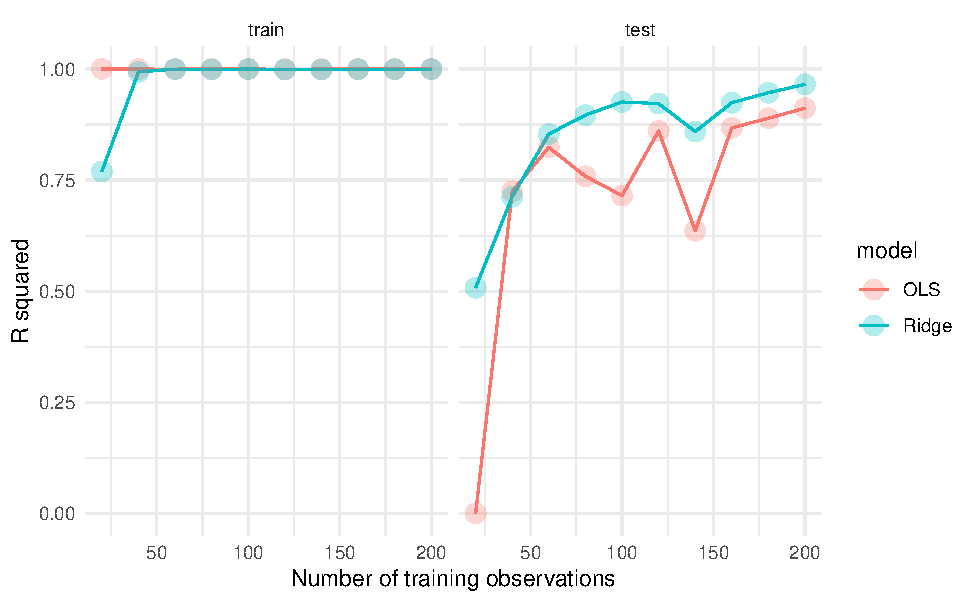
\includegraphics[width=0.8\linewidth]{./figs/unnamed-chunk-1-1} \end{center}

The strength of the ridge regression comes from the fact that it compromises fitting the training data really well for improved generalization. In other words, we increase \textbf{bias} (because we force the coefficients to be smaller) for lower \textbf{variance} (but we make it more general). In other words, the whole gist behind ridge regression is penalizing very large coefficients for better generalization.

Having that intuition in mind, the predictors of the ridge regression need to be standardized. Why is this the case? Because due to the scale of a predictor, its coefficient can be more penalized than other predictors. Suppose that you have the income of a particular person (measured in thousands per months) and time spent with their families (measured in seconds) and you're trying to predict happiness. A one unit increase in salary could be penalized much more than a one unit increase in time spent with their families \textbf{just} because a one unit increase in salary can be much bigger due to it's metric.

In R, you can fit a ridge regression (and nearly all other machine learning models) through the \texttt{caret} package. Let's load the packages that we will work with and read the data:

\begin{Shaded}
\begin{Highlighting}[]
\KeywordTok{library}\NormalTok{(caret) }\CommentTok{# Fitting machine learning models}
\KeywordTok{library}\NormalTok{(rsample) }\CommentTok{# Create data partitions}
\KeywordTok{library}\NormalTok{(vip) }\CommentTok{# For figuring out important variables for prediction}

\NormalTok{data_link <-}\StringTok{ "https://raw.githubusercontent.com/cimentadaj/ml_socsci/master/data/pisa_us_2018.csv"}
\NormalTok{pisa <-}\StringTok{ }\KeywordTok{read.csv}\NormalTok{(data_link)}
\end{Highlighting}
\end{Shaded}

First thing we do is separate the training and test data. All of our modelling will be performed on the training data and the test data is saved for later (the test data must be completely ignored until you have your final tuned model).

\begin{Shaded}
\begin{Highlighting}[]
\CommentTok{# Separate training/testing split}

\CommentTok{# Place a seed for reproducing the results}
\KeywordTok{set.seed}\NormalTok{(}\DecValTok{23141}\NormalTok{)}
\NormalTok{split_pisa <-}\StringTok{ }\KeywordTok{initial_split}\NormalTok{(}\DataTypeTok{data =}\NormalTok{ pisa, }\DataTypeTok{prop =} \FloatTok{.7}\NormalTok{)}
\NormalTok{pisa_test <-}\StringTok{ }\KeywordTok{testing}\NormalTok{(split_pisa)}
\NormalTok{pisa_train <-}\StringTok{ }\KeywordTok{training}\NormalTok{(split_pisa)}
\end{Highlighting}
\end{Shaded}

The ridge regression has a parameter called \texttt{lambda} which needs to be set by us. \texttt{lambda} is the ``weight'' term in the ridge equation, which controls how much weight do we want to give to the ``shrinkage penalty''. If this lambda is 0, it means we attach \textbf{no} weight to the penalty term and we will get the same result over OLS. Let's try that:

\begin{Shaded}
\begin{Highlighting}[]
\CommentTok{############################# Ridge regression ################################}
\CommentTok{###############################################################################}

\NormalTok{ridge_grid <-}\StringTok{ }\KeywordTok{data.frame}\NormalTok{(}
  \CommentTok{# Here we specify the lambda to be zero}
  \DataTypeTok{lambda =} \DecValTok{0}\NormalTok{,}
  \CommentTok{# Here we specify the type of penalized regression: 0 is ridge regression}
  \DataTypeTok{alpha =} \DecValTok{0}
\NormalTok{)}

\CommentTok{# The train function accepts several arguments}
\NormalTok{ridge_mod <-}\StringTok{ }\KeywordTok{train}\NormalTok{(}
  \CommentTok{# math_score is the dependent variable and all other are independent variables}
\NormalTok{  math_score }\OperatorTok{~}\StringTok{ }\NormalTok{MISCED }\OperatorTok{+}\StringTok{ }\NormalTok{FISCED }\OperatorTok{+}\StringTok{ }\NormalTok{HISEI }\OperatorTok{+}\StringTok{ }\NormalTok{REPEAT }\OperatorTok{+}\StringTok{ }\NormalTok{IMMIG }\OperatorTok{+}\StringTok{ }\NormalTok{DURECEC }\OperatorTok{+}\StringTok{ }\NormalTok{BSMJ,}
  \CommentTok{# The training data}
  \DataTypeTok{data =}\NormalTok{ pisa_train,}
  \CommentTok{# The R package that runs the ridge regression}
  \DataTypeTok{method =} \StringTok{"glmnet"}\NormalTok{,}
  \CommentTok{# Here is where we pass the lambda argument}
  \DataTypeTok{tuneGrid =}\NormalTok{ ridge_grid,}
  \DataTypeTok{lambda =} \DecValTok{0}\NormalTok{,}
  \CommentTok{# Here is where the function standardizes the predictors before}
  \CommentTok{# fitting the models}
  \DataTypeTok{preProc =} \KeywordTok{c}\NormalTok{(}\StringTok{"center"}\NormalTok{, }\StringTok{"scale"}\NormalTok{),}
  \DataTypeTok{trControl =} \KeywordTok{trainControl}\NormalTok{(}\DataTypeTok{method =} \StringTok{"none"}\NormalTok{)}
\NormalTok{)}

\CommentTok{# Get ridge coefficients}
\NormalTok{res <-}\StringTok{ }\NormalTok{ridge_mod}\OperatorTok{$}\NormalTok{finalModel}
\NormalTok{ridge_coef <-}\StringTok{ }\KeywordTok{predict}\NormalTok{(res, }\DataTypeTok{s =} \DecValTok{0}\NormalTok{, }\DataTypeTok{type =} \StringTok{"coefficients"}\NormalTok{)}

\CommentTok{############################# Linear model ####################################}
\CommentTok{###############################################################################}

\NormalTok{iv_vars <-}\StringTok{ }\KeywordTok{c}\NormalTok{(}\StringTok{"MISCED"}\NormalTok{, }\StringTok{"FISCED"}\NormalTok{, }\StringTok{"HISEI"}\NormalTok{, }\StringTok{"REPEAT"}\NormalTok{, }\StringTok{"IMMIG"}\NormalTok{, }\StringTok{"DURECEC"}\NormalTok{, }\StringTok{"BSMJ"}\NormalTok{)}
\NormalTok{pisa_tst <-}\StringTok{ }\NormalTok{pisa_train}
\NormalTok{pisa_tst[iv_vars] <-}\StringTok{ }\KeywordTok{scale}\NormalTok{(pisa_tst[iv_vars])}

\NormalTok{lm_coef <-}\StringTok{ }\KeywordTok{coef}\NormalTok{(}
  \KeywordTok{lm}\NormalTok{(math_score }\OperatorTok{~}\StringTok{ }\NormalTok{MISCED }\OperatorTok{+}\StringTok{ }\NormalTok{FISCED }\OperatorTok{+}\StringTok{ }\NormalTok{HISEI }\OperatorTok{+}\StringTok{ }\NormalTok{REPEAT }\OperatorTok{+}\StringTok{ }\NormalTok{IMMIG }\OperatorTok{+}\StringTok{ }\NormalTok{DURECEC }\OperatorTok{+}\StringTok{ }\NormalTok{BSMJ,}
     \DataTypeTok{data =}\NormalTok{ pisa_tst)}
\NormalTok{)}

\CommentTok{############################# Comparing model #################################}
\CommentTok{###############################################################################}

\NormalTok{comparison <-}
\StringTok{  }\KeywordTok{data.frame}\NormalTok{(}\DataTypeTok{coefs =} \KeywordTok{names}\NormalTok{(lm_coef),}
             \StringTok{`}\DataTypeTok{Linear coefficients}\StringTok{`}\NormalTok{ =}\StringTok{ }\KeywordTok{unname}\NormalTok{(}\KeywordTok{round}\NormalTok{(lm_coef, }\DecValTok{2}\NormalTok{)),}
             \StringTok{`}\DataTypeTok{Ridge coefficients}\StringTok{`}\NormalTok{ =}\StringTok{ }\KeywordTok{round}\NormalTok{(}\KeywordTok{as.vector}\NormalTok{(ridge_coef), }\DecValTok{2}\NormalTok{))}

\NormalTok{knitr}\OperatorTok{::}\KeywordTok{kable}\NormalTok{(comparison)}
\end{Highlighting}
\end{Shaded}

\begin{tabular}{l|r|r}
\hline
coefs & Linear.coefficients & Ridge.coefficients\\
\hline
(Intercept) & 473.05 & 473.05\\
\hline
MISCED & 2.94 & 2.94\\
\hline
FISCED & 11.78 & 11.78\\
\hline
HISEI & 18.07 & 18.07\\
\hline
REPEAT & -22.09 & -22.09\\
\hline
IMMIG & 6.01 & 6.01\\
\hline
DURECEC & 0.55 & 0.55\\
\hline
BSMJ & 10.62 & 10.62\\
\hline
\end{tabular}

Coming from a social science background, it might seem counterintuitive that the researcher has to specify tuning parameters for the model. In traditional social science statistics, models usually estimate similar values internally and the user doesn't have to think about them. However, there are strategies already implemented to explore the combination of many possible values. With our previous example, we just have to add a number of lambda values and \texttt{train} will find the best one:

\begin{Shaded}
\begin{Highlighting}[]
\KeywordTok{set.seed}\NormalTok{(}\DecValTok{663421}\NormalTok{)}

\NormalTok{ridge_grid <-}\StringTok{ }\KeywordTok{data.frame}\NormalTok{(}
  \CommentTok{# Here we specify the lambda to several possible values}
  \DataTypeTok{lambda =} \KeywordTok{seq}\NormalTok{(}\DecValTok{0}\NormalTok{, }\DecValTok{3}\NormalTok{, }\DataTypeTok{length.out =} \DecValTok{300}\NormalTok{),}
  \CommentTok{# Here we specify the type of penalized regression: 0 is ridge regression}
  \DataTypeTok{alpha =} \DecValTok{0}
\NormalTok{)}

\NormalTok{ridge_mod <-}\StringTok{ }\KeywordTok{train}\NormalTok{(}
\NormalTok{  math_score }\OperatorTok{~}\StringTok{ }\NormalTok{MISCED }\OperatorTok{+}\StringTok{ }\NormalTok{FISCED }\OperatorTok{+}\StringTok{ }\NormalTok{HISEI }\OperatorTok{+}\StringTok{ }\NormalTok{REPEAT }\OperatorTok{+}\StringTok{ }\NormalTok{IMMIG }\OperatorTok{+}\StringTok{ }\NormalTok{DURECEC }\OperatorTok{+}\StringTok{ }\NormalTok{BSMJ,}
  \DataTypeTok{data =}\NormalTok{ pisa_train,}
  \DataTypeTok{method =} \StringTok{"glmnet"}\NormalTok{,}
  \DataTypeTok{tuneGrid =}\NormalTok{ ridge_grid,}
  \DataTypeTok{preProc =} \KeywordTok{c}\NormalTok{(}\StringTok{"center"}\NormalTok{, }\StringTok{"scale"}\NormalTok{),}
  \CommentTok{# Performs cross validation through all grid parameters}
  \DataTypeTok{trControl =} \KeywordTok{trainControl}\NormalTok{(}\DataTypeTok{method =} \StringTok{"cv"}\NormalTok{, }\DataTypeTok{number =} \DecValTok{5}\NormalTok{)}
\NormalTok{)}

\KeywordTok{plot}\NormalTok{(ridge_mod}\OperatorTok{$}\NormalTok{finalModel, }\DataTypeTok{xvar =} \StringTok{"lambda"}\NormalTok{, }\DataTypeTok{label =} \OtherTok{TRUE}\NormalTok{)}
\end{Highlighting}
\end{Shaded}

\begin{center}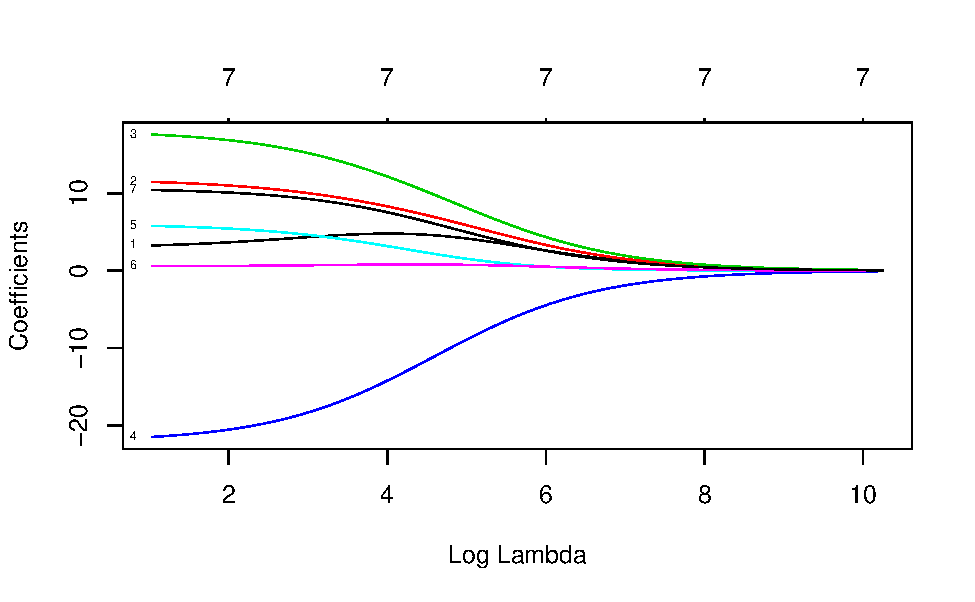
\includegraphics[width=0.8\linewidth]{./figs/unnamed-chunk-5-1} \end{center}

Here we can see how our coefficients are affected by increasing weight of the \texttt{lambda} parameter. And we can figure out the best lambda inspecting \texttt{bestTune} inside \texttt{ridge\_mod}:

\begin{Shaded}
\begin{Highlighting}[]
\NormalTok{best_lambda_ridge <-}\StringTok{ }\NormalTok{ridge_mod}\OperatorTok{$}\NormalTok{bestTune}\OperatorTok{$}\NormalTok{lambda}
\NormalTok{best_lambda_ridge}
\end{Highlighting}
\end{Shaded}

\begin{verbatim}
## [1] 2.67893
\end{verbatim}

However, there's no need to rerun the model with this optimal value; since \texttt{train} \textbf{had} to run that model, it saves it as the most optimal:

\begin{Shaded}
\begin{Highlighting}[]
\NormalTok{holdout_ridge <-}
\StringTok{  }\KeywordTok{RMSE}\NormalTok{(}
    \KeywordTok{predict}\NormalTok{(ridge_mod, pisa_test, }\DataTypeTok{s =}\NormalTok{ best_lambda_ridge),}
\NormalTok{    pisa_test}\OperatorTok{$}\NormalTok{math_score}
\NormalTok{  )}

\NormalTok{train_rmse_ridge <-}
\StringTok{  }\NormalTok{ridge_mod}\OperatorTok{$}\NormalTok{results }\OperatorTok
\StringTok{  }\KeywordTok{filter}\NormalTok{(lambda }\OperatorTok{==}\StringTok{ }\NormalTok{best_lambda_ridge) }\OperatorTok
\StringTok{  }\KeywordTok{pull}\NormalTok{(RMSE)}

\KeywordTok{c}\NormalTok{(}\DataTypeTok{holdout_rmse =}\NormalTok{ holdout_ridge, }\DataTypeTok{train_rmse =}\NormalTok{ train_rmse_ridge)}
\end{Highlighting}
\end{Shaded}

\begin{verbatim}
## holdout_rmse   train_rmse 
##     79.11585     76.37490
\end{verbatim}

The holdout RMSE will always be higher than the training RMSE as the training set nearly always \textbf{memorizes} the data better for the training.

\hypertarget{lasso-regularization}{%
\section{Lasso regularization}\label{lasso-regularization}}

The Lasso regularization is very similar to the ridge regularization where only one thing changes: the penalty term. Instead of squaring the coefficients in the penalty term, the lasso regularization takes the absolute value of the coefficient.

\begin{equation}
RSS + \lambda \sum_{k = 1}^n |\beta_j|
\end{equation}

Althought it might not be self-evident from this, the lasso reguralization has an important distinction: it can force a coefficient to be zero. This means that lasso does a selection of variables which have big coefficients while not compromising the RSS of the model. The problem with ridge regression is that as the number of variables increases, the training error will almost always decrease but the test error will not.

For example, if we define the same model from above using a lasso, you'll see that it forces coefficients to be \textbf{exactly zero} if they don't add anything relative to the RSS of the model. This means that variables which do not add anything to the model will be excluded unless they add explanatory power that compensates the size of their coefficient. Here's the same lasso example:

\begin{Shaded}
\begin{Highlighting}[]
\KeywordTok{set.seed}\NormalTok{(}\DecValTok{663421}\NormalTok{)}

\NormalTok{lasso_grid <-}\StringTok{ }\KeywordTok{data.frame}\NormalTok{(}
  \CommentTok{# Here we specify the lambda to several possible values}
  \DataTypeTok{lambda =} \KeywordTok{seq}\NormalTok{(}\DecValTok{0}\NormalTok{, }\DecValTok{3}\NormalTok{, }\DataTypeTok{length.out =} \DecValTok{300}\NormalTok{),}
  \CommentTok{# Here we specify the type of penalized regression: 1 is lasso regression}
  \DataTypeTok{alpha =} \DecValTok{1}
\NormalTok{)}

\NormalTok{lasso_mod <-}\StringTok{ }\KeywordTok{train}\NormalTok{(}
\NormalTok{  math_score }\OperatorTok{~}\StringTok{ }\NormalTok{MISCED }\OperatorTok{+}\StringTok{ }\NormalTok{FISCED }\OperatorTok{+}\StringTok{ }\NormalTok{HISEI }\OperatorTok{+}\StringTok{ }\NormalTok{REPEAT }\OperatorTok{+}\StringTok{ }\NormalTok{IMMIG }\OperatorTok{+}\StringTok{ }\NormalTok{DURECEC }\OperatorTok{+}\StringTok{ }\NormalTok{BSMJ,}
  \DataTypeTok{data =}\NormalTok{ pisa_train,}
  \DataTypeTok{method =} \StringTok{"glmnet"}\NormalTok{,}
  \DataTypeTok{tuneGrid =}\NormalTok{ lasso_grid,}
  \DataTypeTok{preProc =} \KeywordTok{c}\NormalTok{(}\StringTok{"center"}\NormalTok{, }\StringTok{"scale"}\NormalTok{),}
  \DataTypeTok{trControl =} \KeywordTok{trainControl}\NormalTok{(}\DataTypeTok{method =} \StringTok{"cv"}\NormalTok{)}
\NormalTok{)}

\KeywordTok{plot}\NormalTok{(lasso_mod}\OperatorTok{$}\NormalTok{finalModel, }\DataTypeTok{xvar =} \StringTok{"lambda"}\NormalTok{, }\DataTypeTok{label =} \OtherTok{TRUE}\NormalTok{)}
\end{Highlighting}
\end{Shaded}

\begin{center}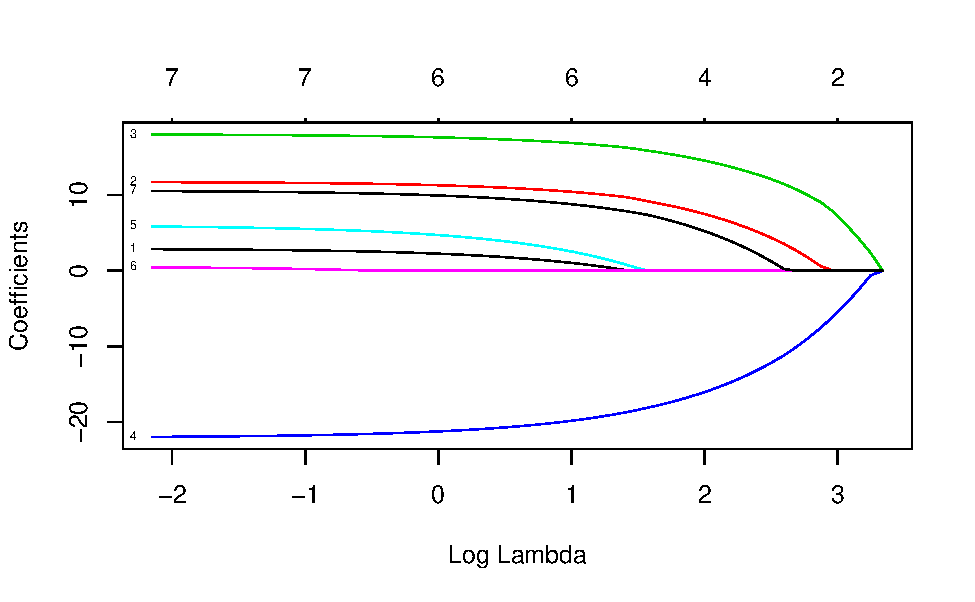
\includegraphics[width=0.8\linewidth]{./figs/unnamed-chunk-8-1} \end{center}

In contrast to the ridge regression, where coefficients are forced to be close to zero, the lasso penalty actually forces some coefficients \textbf{to be zero}. This property means that the lasso makes a \textbf{selection of the variables with the higher coefficients} and eliminates those which do not have a strong relationship. Lasso is usually better at model interpretation because it removes redundant variables while ridge can be useful if you want to keep a number of variables in the model, despite them being weak predictors (as controls, for example).

The lasso actually works exactly as the ridge in the \texttt{caret} package, meaning that it automatically checks the most optimal value for lambda:

\begin{Shaded}
\begin{Highlighting}[]
\NormalTok{best_lambda_lasso <-}\StringTok{ }\NormalTok{lasso_mod}\OperatorTok{$}\NormalTok{bestTune}\OperatorTok{$}\NormalTok{lambda}
\NormalTok{best_lambda_lasso}
\end{Highlighting}
\end{Shaded}

\begin{verbatim}
## [1] 0.1906355
\end{verbatim}

To actually check the final model and which variables are kept, we can access it:

\begin{Shaded}
\begin{Highlighting}[]
\NormalTok{holdout_lasso <-}
\StringTok{  }\KeywordTok{RMSE}\NormalTok{(}
    \KeywordTok{predict}\NormalTok{(lasso_mod, pisa_test, }\DataTypeTok{s =}\NormalTok{ best_lambda_lasso),}
\NormalTok{    pisa_test}\OperatorTok{$}\NormalTok{math_score}
\NormalTok{  )}

\NormalTok{train_rmse_lasso <-}
\StringTok{  }\NormalTok{lasso_mod}\OperatorTok{$}\NormalTok{results }\OperatorTok
\StringTok{  }\KeywordTok{filter}\NormalTok{(lambda }\OperatorTok{==}\StringTok{ }\NormalTok{best_lambda_lasso) }\OperatorTok
\StringTok{  }\KeywordTok{pull}\NormalTok{(RMSE)}

\KeywordTok{c}\NormalTok{(}\DataTypeTok{holdout_rmse =}\NormalTok{ holdout_lasso, }\DataTypeTok{train_rmse =}\NormalTok{ train_rmse_lasso)}
\end{Highlighting}
\end{Shaded}

\begin{verbatim}
## holdout_rmse   train_rmse 
##     79.13141     76.31036
\end{verbatim}

So far, we can check which model is performing better:

\begin{Shaded}
\begin{Highlighting}[]
\NormalTok{model_comparison <-}
\StringTok{  }\KeywordTok{data.frame}\NormalTok{(}
    \DataTypeTok{type =} \KeywordTok{c}\NormalTok{(}\StringTok{"test RMSE"}\NormalTok{, }\StringTok{"training RMSE"}\NormalTok{),}
    \DataTypeTok{ridge =} \KeywordTok{c}\NormalTok{(holdout_ridge, train_rmse_ridge),}
    \DataTypeTok{lasso =} \KeywordTok{c}\NormalTok{(holdout_lasso, train_rmse_lasso)}
\NormalTok{  )}

\NormalTok{model_comparison}
\end{Highlighting}
\end{Shaded}

\begin{verbatim}
##            type    ridge    lasso
## 1     test RMSE 79.11585 79.13141
## 2 training RMSE 76.37490 76.31036
\end{verbatim}

Currently the ridge regression has a very minor advantaged over the lasso yet the difference is probably within the margin of error. Depending on your aim, you might want to choose either of the models. For example, if our models contained a lot of variables, lasso might be more interpretable as it reduces the number of variables. However, if you have reasons to believe that keeping all variables in the model is important, then ridge provides an advantage.

\hypertarget{elastic-net-regularization}{%
\section{Elastic Net regularization}\label{elastic-net-regularization}}

If you're aware of ridge and lasso, then elastic net regularization is a logical step. Elastic Net (the name sounds fancy, but it is also an adaptation of OLS) combines both penalties to form one single equation.

Here we define our ridge penalty:

\[ridge = \lambda \sum_{k = 1}^n |\beta_j|\]

And here we define our lasso penalty:

\[lasso = \lambda \sum_{k = 1}^n \beta_j^2\]

Elastic net regularization is the addition of these two penalties in comparison to the RSS:

\[RSS + lasso + ridge\]

I think the best explanation for elastic net reguarlization comes from Boehmke \& Greenwell (2019):

\begin{quote}
Although lasso models perform feature selection, when two strongly correlated features are pushed towards zero, one may be pushed fully to zero while the other remains in the model. Furthermore, the process of one being in and one being out is not very systematic. In contrast, the ridge regression penalty is a little more effective in systematically handling correlated features together. Consequently, the advantage of the elastic net penalty is that it enables effective regularization via the ridge penalty with the feature selection characteristics of the lasso penalty.
\end{quote}

Essentially, you now have two tuning parameters. In the grid of values, instead of specifying an alpha of \texttt{0} (ridge) or \texttt{1} (lasso), \texttt{caret} will slide through several values of \texttt{alpha} ranging from 0 to 1 and compare that to several values of \texttt{lambda}.

However, \texttt{train} can already take care of this and calculate the most optimal value automatically with specifying a grid of values:

\begin{Shaded}
\begin{Highlighting}[]
\KeywordTok{set.seed}\NormalTok{(}\DecValTok{663421}\NormalTok{)}

\NormalTok{elnet_mod <-}\StringTok{ }\KeywordTok{train}\NormalTok{(}
\NormalTok{  math_score }\OperatorTok{~}\StringTok{ }\NormalTok{MISCED }\OperatorTok{+}\StringTok{ }\NormalTok{FISCED }\OperatorTok{+}\StringTok{ }\NormalTok{HISEI }\OperatorTok{+}\StringTok{ }\NormalTok{REPEAT }\OperatorTok{+}\StringTok{ }\NormalTok{IMMIG }\OperatorTok{+}\StringTok{ }\NormalTok{DURECEC }\OperatorTok{+}\StringTok{ }\NormalTok{BSMJ,}
  \DataTypeTok{data =}\NormalTok{ pisa_train,}
  \DataTypeTok{method =} \StringTok{"glmnet"}\NormalTok{,}
  \DataTypeTok{preProc =} \KeywordTok{c}\NormalTok{(}\StringTok{"center"}\NormalTok{, }\StringTok{"scale"}\NormalTok{),}
  \DataTypeTok{trControl =} \KeywordTok{trainControl}\NormalTok{(}\DataTypeTok{method =} \StringTok{"cv"}\NormalTok{),}
  \CommentTok{# Here 25 means that it will try 25 values of}
  \CommentTok{# alpha and then N numbers of alpha}
  \DataTypeTok{tuneLength =} \DecValTok{25}
\NormalTok{)}

\NormalTok{best_lambda_elnet <-}\StringTok{ }\NormalTok{elnet_mod}\OperatorTok{$}\NormalTok{bestTune}\OperatorTok{$}\NormalTok{lambda}

\NormalTok{holdout_elnet <-}
\StringTok{  }\KeywordTok{RMSE}\NormalTok{(}
    \KeywordTok{predict}\NormalTok{(elnet_mod, pisa_test),}
\NormalTok{    pisa_test}\OperatorTok{$}\NormalTok{math_score}
\NormalTok{  )}

\NormalTok{train_rmse_elnet <-}
\StringTok{  }\NormalTok{elnet_mod}\OperatorTok{$}\NormalTok{results }\OperatorTok
\StringTok{  }\KeywordTok{filter}\NormalTok{(alpha }\OperatorTok{==}\StringTok{ }\NormalTok{elnet_mod}\OperatorTok{$}\NormalTok{bestTune}\OperatorTok{$}\NormalTok{alpha, lambda }\OperatorTok{==}\StringTok{ }\NormalTok{best_lambda_elnet) }\OperatorTok
\StringTok{  }\KeywordTok{pull}\NormalTok{(RMSE)}

\KeywordTok{c}\NormalTok{(}\DataTypeTok{holdout_rmse =}\NormalTok{ holdout_elnet, }\DataTypeTok{train_rmse =}\NormalTok{ train_rmse_elnet)}
\end{Highlighting}
\end{Shaded}

\begin{verbatim}
## holdout_rmse   train_rmse 
##     79.12763     76.31005
\end{verbatim}

The RMSE of the elastic net is somewhat lower than then ridge and lasso but also probably within the margin of error. Let's compare it visually:

\begin{Shaded}
\begin{Highlighting}[]
\NormalTok{model_comparison}\OperatorTok{$}\NormalTok{elnet <-}\StringTok{ }\KeywordTok{c}\NormalTok{(holdout_elnet, train_rmse_elnet)}
\NormalTok{model_comparison}
\end{Highlighting}
\end{Shaded}

\begin{verbatim}
##            type    ridge    lasso    elnet
## 1     test RMSE 79.11585 79.13141 79.12763
## 2 training RMSE 76.37490 76.31036 76.31005
\end{verbatim}

\begin{Shaded}
\begin{Highlighting}[]
\NormalTok{model_comparison }\OperatorTok
\StringTok{  }\KeywordTok{pivot_longer}\NormalTok{(}\OperatorTok{-}\NormalTok{type) }\OperatorTok
\StringTok{  }\KeywordTok{ggplot}\NormalTok{(}\KeywordTok{aes}\NormalTok{(name, value, }\DataTypeTok{color =}\NormalTok{ type, }\DataTypeTok{group =}\NormalTok{ type)) }\OperatorTok{+}
\StringTok{  }\KeywordTok{geom_point}\NormalTok{(}\DataTypeTok{position =} \StringTok{"dodge"}\NormalTok{) }\OperatorTok{+}
\StringTok{  }\KeywordTok{geom_line}\NormalTok{() }\OperatorTok{+}
\StringTok{  }\KeywordTok{scale_y_continuous}\NormalTok{(}\DataTypeTok{name =} \StringTok{"RMSE"}\NormalTok{) }\OperatorTok{+}
\StringTok{  }\KeywordTok{scale_x_discrete}\NormalTok{(}\DataTypeTok{name =} \StringTok{"Models"}\NormalTok{) }\OperatorTok{+}
\StringTok{  }\KeywordTok{theme_minimal}\NormalTok{()}
\end{Highlighting}
\end{Shaded}

\begin{center}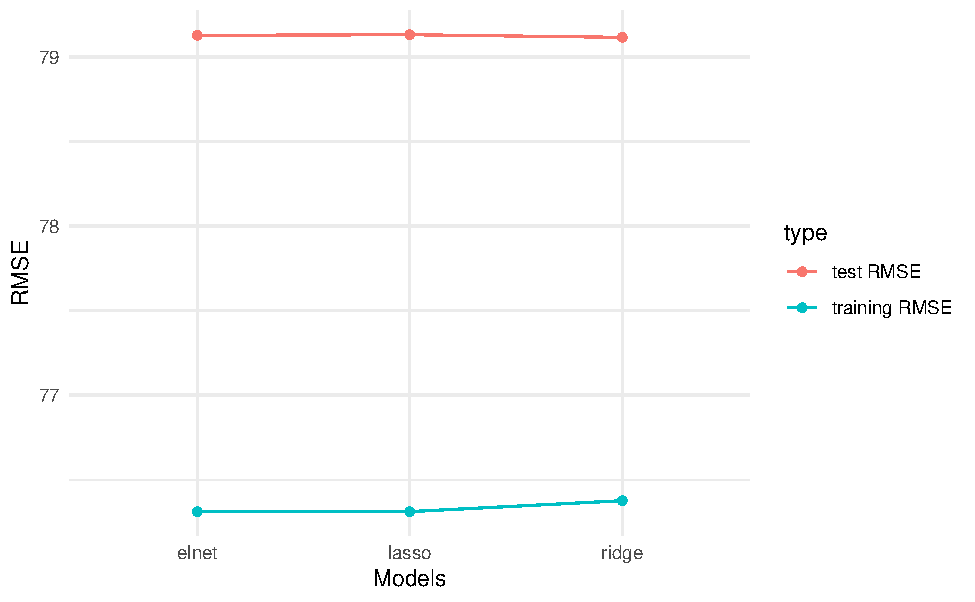
\includegraphics[width=0.8\linewidth]{./figs/unnamed-chunk-13-1} \end{center}

\hypertarget{exercises}{%
\section{Exercises}\label{exercises}}

The \href{https://www.fragilefamilieschallenge.org/}{Fragile Families Challenge} is a study that aimed to predict a series of indicators of children at age 15 only using data from ages 0 to 9. With this challenge, the principal investigators wanted to test whether skills such as cognitive and non-cognitive abilities were correctly predicted. With that idea in mind, they were interested in following up children that beat the `predictions': those children that exceeded the model's prediction, for example given their initial conditions.

Using a similarly constructed non-cognitive proxy, I've created a non-cognitive index using the PISA 2018 for the United States which is the average of the questions:

\begin{itemize}
\tightlist
\item
  ST182Q03HA - I find satisfaction in working as hard as I can.
\item
  ST182Q04HA - Once I start a task, I persist until it is finished.
\item
  ST182Q05HA - Part of the enjoyment I get from doing things is when I improve on my past performance.
\item
  ST182Q06HA - If I am not good at something, I would rather keep struggling to master it than move on to something I may {[}\ldots{]}
\end{itemize}

The scale of the index goes from 1 to 4, where 4 the student strongly agrees and 1 is they completely disagree. In other words, this index shows that the higher the value, the higher the non cognitive skills. You can check out the complete PISA codebook \href{https://docs.google.com/spreadsheets/d/12--3vD737rcu6olviKutRLEiyKNZ2bynXcJ4CpwtNsQ/edit?usp=sharing}{here}.

In these series of exercises you will have to try different models that predict this index of non-cognitive skills, choose the best model and look at the most important variables.

First, read in the data with:

\begin{Shaded}
\begin{Highlighting}[]
\NormalTok{data_link <-}\StringTok{ "https://raw.githubusercontent.com/cimentadaj/ml_socsci/master/data/pisa_us_2018.csv"}
\NormalTok{pisa <-}\StringTok{ }\KeywordTok{read.csv}\NormalTok{(data_link)}
\end{Highlighting}
\end{Shaded}

\hypertarget{split-the-data-into-testtraining-data}{%
\subsection{Split the data into test/training data}\label{split-the-data-into-testtraining-data}}

Remember to set the seed to \texttt{2341} so that everyone can compare their results.

\hypertarget{run-a-ridge-regression-with-non-cognitive-as-the-dependent-variable}{%
\subsection{Run a ridge regression with non-cognitive as the dependent variable}\label{run-a-ridge-regression-with-non-cognitive-as-the-dependent-variable}}

Use as many variables as you want (you can reuse the previous variables from the examples or pick all of them). A formula of the like \texttt{noncogn\ \textasciitilde{}\ .} will regress \texttt{noncogn} on all variables.

\begin{Shaded}
\begin{Highlighting}[]
\CommentTok{# 1) Define ridge grid of values for lambda}
\NormalTok{ridge_grid <-}\StringTok{ }\KeywordTok{data.frame}\NormalTok{(}
  \DataTypeTok{lambda =} 
  \DataTypeTok{alpha =} \DecValTok{0}
\NormalTok{)}

\CommentTok{# 2) Use the train function to train the model on the *training set*}

\CommentTok{# 3) Extract the best lambda and calculate the RMSE on the test set}

\CommentTok{# 4) Extract the RMSE of the training set}

\CommentTok{# 5) Compare both holdout and training RMSE}
\end{Highlighting}
\end{Shaded}

\hypertarget{which-are-the-most-important-variables}{%
\subsection{Which are the most important variables?}\label{which-are-the-most-important-variables}}

Comment on their coefficients and whether they make sense to be included in the model.

\hypertarget{run-a-lasso-regression-with-the-same-specification-as-above}{%
\subsection{Run a lasso regression with the same specification as above}\label{run-a-lasso-regression-with-the-same-specification-as-above}}

\begin{Shaded}
\begin{Highlighting}[]
\CommentTok{# Define ridge grid of values for lambda}
\NormalTok{lasso_grid <-}\StringTok{ }\KeywordTok{data.frame}\NormalTok{(}
  \DataTypeTok{lambda =} 
  \DataTypeTok{alpha =} \DecValTok{1}
\NormalTok{)}

\CommentTok{# Reproduce previous steps}
\end{Highlighting}
\end{Shaded}

Which model is performing better? Ridge or Lasso? Are the same variables the strongest predictors across models? Which variables are the strongest predictors?

\hypertarget{run-an-elastic-net-regression-on-non-cognitive-skills}{%
\subsection{Run an elastic net regression on non cognitive skills}\label{run-an-elastic-net-regression-on-non-cognitive-skills}}

Since \texttt{train} already takes care of trying all possible values, there's no need to pass a grid of lambda values. It is only needed to set the \texttt{tuneLength} to a number of alpha values.

\hypertarget{compare-the-three-models-graphically}{%
\subsection{Compare the three models graphically}\label{compare-the-three-models-graphically}}

\begin{itemize}
\tightlist
\item
  Comment on which models is better in out-of-sample fit
\item
  Is it better to keep the most accurate model or a model that includes relevant confounders (even if they're relationship is somewhat weak)?
\end{itemize}

You can find the answer to all problems \href{./answers/02_regularization.R}{here}

\hypertarget{bibliography}{%
\section{Bibliography}\label{bibliography}}

Boehmke, B., \& Greenwell, B. M. (2019). Hands-On Machine Learning with R. CRC Press.

Friedman, J., Hastie, T., \& Tibshirani, R. (2001). The elements of statistical learning (Vol. 1, No.~10). New York: Springer series in statistics.

\hypertarget{syllabus}{%
\chapter{Syllabus}\label{syllabus}}

\hypertarget{course-description}{%
\section{Course description}\label{course-description}}

With the increasing amounts of data being collected on a daily basis, the field of machine learning has gained mainstream attention. By shifting away from focusing on inference, machine learning is a field at the intersection of statistics and computer science that is focused on maximizing predictive performance by learning patterns from data. That is, the goal of machine learning is to predict something -- and predict it very well, regardless of whether you understand it. These techniques are common in business settings where, for example, stakeholders are interested in knowing the probability of a client leaving a company or the propensity of a client for buying a particular product. The field can be intimidating as it is vast and growing every year.

However, scholars in the social sciences are beginning to understand the importance of the machine learning framework and how it can unlock new knowledge in fields such as sociology, political science, economics and psychology. On this course we will introduce students to the basic ideas of the machine learning framework and touch upon the basic algorithms used for prediction and discussing the potential it can have in the social sciences.

In particular, we will introduce predictive algorithms such as regularized regressions, classification trees and clustering techniques through basic examples. We will discuss their advantages and disadvantages while paying great attention to how it's been used in research. Although many social scientists do not see how predictive models can help explain social phenomena, we will also focus on how machine learning can play a role as a tool for discovery, improving causal inference and generalizing our classical models through cross validation.

We will end the course with a prediction challenge that will put to test all of your acquired knowledge. Starting with a discussion on the role of predictive challenges such as the \href{http://www.fragilefamilieschallenge.org/}{Fragile Families Challenge} in the social sciences, our predictive challenge will require the student to run machine learning algorithms, test their out-of-sample error rate and discuss strategies on how the results are useful. This will give the class a real hands-on example of how to incorporate machine learning into their research right away. Below is a detailed description of the syllabus.

\hypertarget{schedule}{%
\section{Schedule}\label{schedule}}

\textbf{Session 1}\\
\textbf{July 6th 09:00h-10:45h}

\begin{itemize}
\tightlist
\item
  Introduction to the Machine Learning Framework

  \begin{itemize}
  \tightlist
  \item
    Inference vs Prediction
  \item
    Can inference and prediction complement each other?
  \item
    Bias-variance / Interpretability-prediction tradeoffs
  \item
    Resampling for understtanding your model
  \item
    ``\href{http://www.fragilefamilieschallenge.org/}{The Fragile Families Challenge}''
  \end{itemize}
\end{itemize}

\textbf{Readings}:

\begin{itemize}
\item
  Sections 2.1 and 2.2 from James, Gareth, et al.~An Introduction To Statistical Learning. Vol. 112. New York: springer, 2013
\item
  Molina, M., \& Garip, F. (2019). Machine Learning for Sociology. Annual Review of Sociology, 45.
\item
  Mullainathan, S., \& Spiess, J. (2017). Machine learning: an applied econometric approach. Journal of Economic Perspectives, 31(2), 87-106.
\item
  Breiman, L. (2001). Statistical modeling: The two cultures (with comments and a rejoinder by the author). Statistical science, 16(3), 199-231.
\end{itemize}

\begin{center}\rule{0.5\linewidth}{\linethickness}\end{center}

\textbf{Break 10:45h-11:15h}

\begin{center}\rule{0.5\linewidth}{\linethickness}\end{center}

\textbf{Session 2}\\
\textbf{July 6th 11:15h-13:00h}

\begin{itemize}
\tightlist
\item
  Linear regression and regularization

  \begin{itemize}
  \tightlist
  \item
    Continuous predictions and loss functions
  \item
    Lasso

    \begin{itemize}
    \tightlist
    \item
      Advantages/Disadvantages
    \item
      R example
    \end{itemize}
  \item
    Ridge regression

    \begin{itemize}
    \tightlist
    \item
      Advantages/Disadvantages
    \item
      R example
    \end{itemize}
  \item
    Elastic Net

    \begin{itemize}
    \tightlist
    \item
      Advantages/Disadvantages
    \item
      R example
    \end{itemize}
  \end{itemize}
\item
  Exercises
\end{itemize}

\textbf{Readings}:

\begin{itemize}
\item
  For a theoretical introduction to Lasso/Ridge, sections 6.1, 6.2 and 6.6 from \emph{James, Gareth, et al.~(2013) An Introduction To Statistical Learning. Vol. 112. New York: springer}
\item
  For hands-on examples, Chapter 6 of \emph{Boehmke \& Greenwell (2019) Hands-On Machine Learning with R, 1st Edition, Chapman \& Hall/CRC The R Series. Accessible at: \url{https://bradleyboehmke.github.io/HOML/}}
\end{itemize}

\textbf{Session 3}\\
\textbf{July 7th 09:00h-10:45h}

\begin{itemize}
\tightlist
\item
  Supervised Regression

  \begin{itemize}
  \tightlist
  \item
    Introduction to supervised regression
  \item
    Classification

    \begin{itemize}
    \tightlist
    \item
      Confusion matrices
    \item
      ROC Curves
    \end{itemize}
  \item
    Classification Trees

    \begin{itemize}
    \tightlist
    \item
      Advantages/Disadvantages
    \item
      R example\\
    \end{itemize}
  \end{itemize}
\item
  Exercises
\end{itemize}

\textbf{Readings}:

\begin{itemize}
\item
  For an introduction to classification trees, Section 8.1, 8.3.1 and 8.3.2 from \emph{James, Gareth, et al.~An Introduction To Statistical Learning. Vol. 112. New York: springer, 2013}
\item
  For hands-on examples, chapter 9 from \emph{Boehmke \& Greenwell (2019) Hands-On Machine Learning with R, 1st Edition, Chapman \& Hall/CRC The R Series. Accessible at: \url{https://bradleyboehmke.github.io/HOML/}}
\item
  For real-world applications of Classification Trees:

  \begin{itemize}
  \item
    Billari, F. C., Fürnkranz, J., \& Prskawetz, A. (2006). Timing, sequencing, and quantum of life course events: A machine learning approach. European Journal of Population/Revue Européenne de Démographie, 22(1), 37-65.
  \item
    Chapter 3 of Nolan, D., \& Lang, D. T. (2015). Data science in R: a case studies approach to computational reasoning and problem solving. CRC Press.
  \end{itemize}
\end{itemize}

\begin{center}\rule{0.5\linewidth}{\linethickness}\end{center}

\textbf{Break 10:45h-11:15h}

\begin{center}\rule{0.5\linewidth}{\linethickness}\end{center}

\textbf{Session 4}\\
\textbf{July 7th 11:15h-13:00h}

\begin{itemize}
\tightlist
\item
  Supervised Regression

  \begin{itemize}
  \tightlist
  \item
    Bagging

    \begin{itemize}
    \tightlist
    \item
      Advantages/Disadvantages
    \item
      R example
    \end{itemize}
  \item
    Random Forest

    \begin{itemize}
    \tightlist
    \item
      Advantages/Disadvantages
    \item
      R example
    \end{itemize}
  \item
    Gradient Boosting

    \begin{itemize}
    \tightlist
    \item
      Advantages/Disadvantages
    \item
      R example
    \end{itemize}
  \end{itemize}
\item
  Exercises
\end{itemize}

\textbf{Readings}:

\begin{itemize}
\item
  For an introduction to bagging/random forests/boosting, Chapter 8 from \emph{James, Gareth, et al.~An Introduction To Statistical Learning. Vol. 112. New York: springer, 2013}
\item
  For hands-on examples, chapter 10, 11 and 12 from \emph{Boehmke \& Greenwell (2019) Hands-On Machine Learning with R, 1st Edition, Chapman \& Hall/CRC The R Series. Accessible at: \url{https://bradleyboehmke.github.io/HOML/}}
\item
  For real-world applications of Random Forests:

  \begin{itemize}
  \item
    Perry, C. (2013). Machine learning and conflict prediction: a use case. Stability: International Journal of Security and Development, 2(3), 56.
  \item
    Berk, R. A., Sorenson, S. B., \& Barnes, G. (2016). Forecasting domestic violence: A machine learning approach to help inform arraignment decisions. Journal of Empirical Legal Studies, 13(1), 94-115.
  \end{itemize}
\end{itemize}

\textbf{Session 5}\\
\textbf{July 8th 09h-10:45h}

\begin{itemize}
\tightlist
\item
  Unsupervised Regression

  \begin{itemize}
  \tightlist
  \item
    Introduction to unsupervised learning
  \item
    Principal Component Analysis (PCA)

    \begin{itemize}
    \tightlist
    \item
      Advantages/Disadvantages
    \item
      R example
    \end{itemize}
  \item
    K-Means clustering

    \begin{itemize}
    \tightlist
    \item
      Advantages/Disadvantages
    \item
      R example
    \end{itemize}
  \end{itemize}
\item
  Exercises
\end{itemize}

\textbf{Readings}:

\begin{itemize}
\item
  For an introduction to unsupervised learning, Section 10.1 from \emph{James, Gareth, et al.~An Introduction To Statistical Learning. Vol. 112. New York: springer, 2013}
\item
  For an introduction to PCA

  \begin{itemize}
  \item
    Section 10.2 and 10.4 from \emph{James, Gareth, et al.~An Introduction To Statistical Learning. 112. New York: springer, 2013}
  \item
    For hands-on examples, chapter 17 from \emph{Boehmke \& Greenwell (2019) Hands-On Machine Learning with R, 1st Edition, Chapman \& Hall/CRC The R Series. Accessible at: \url{https://bradleyboehmke.github.io/HOML/}}
  \end{itemize}
\item
  For an introduction to K-Means clustering

  \begin{itemize}
  \item
    Section 10.5 from \emph{James, Gareth, et al.~An Introduction To Statistical Learning. Vol. 112. New York: springer, 2013}
  \item
    For hands-on examples, chapter 20 from \emph{Boehmke \& Greenwell (2019) Hands-On Machine Learning with R, 1st Edition, Chapman \& Hall/CRC The R Series. Accessible at: \url{https://bradleyboehmke.github.io/HOML/}}
  \end{itemize}
\item
  For real-world applications of K-means clustering:

  \begin{itemize}
  \item
    Garip, F. (2012). Discovering diverse mechanisms of migration: The Mexico--US Stream 1970--2000. Population and Development Review, 38(3), 393-433.
  \item
    Bail, C. A. (2008). The configuration of symbolic boundaries against immigrants in Europe. American Sociological Review, 73(1), 37-59.
  \end{itemize}
\end{itemize}

\begin{center}\rule{0.5\linewidth}{\linethickness}\end{center}

\textbf{Break 10:45h-11:15h}

\begin{center}\rule{0.5\linewidth}{\linethickness}\end{center}

\textbf{Session 6}\\
\textbf{July 8th 11:15h-13:00h}

\begin{itemize}
\tightlist
\item
  Unsupervised Regression

  \begin{itemize}
  \tightlist
  \item
    Hierarchical clustering

    \begin{itemize}
    \tightlist
    \item
      Advantages/Disadvantages
    \item
      R example
    \end{itemize}
  \end{itemize}
\item
  Final challenge: Prediction competition

  \begin{itemize}
  \tightlist
  \item
    Explanation of strategies
  \item
    No free lunch theorem
  \item
    Presentation of results
  \end{itemize}
\end{itemize}

\textbf{Readings}:

\begin{itemize}
\item
  For an introduction to hierarchical clustering, sections 10.3.2, 10.3.3, 10.5.2 from \emph{James, Gareth, et al.~An Introduction To Statistical Learning. Vol. 112. New York: springer, 2013}
\item
  For hands-on examples, chapter 21 from \emph{Boehmke \& Greenwell (2019) Hands-On Machine Learning with R, 1st Edition, Chapman \& Hall/CRC The R Series. Accessible at: \url{https://bradleyboehmke.github.io/HOML/}}
\item
  For examples on prediction competitions:

  \begin{itemize}
  \item
    Glaeser, E. L., Hillis, A., Kominers, S. D., \& Luca, M. (2016). Crowdsourcing city government: Using tournaments to improve inspection accuracy. American Economic Review, 106(5), 114-18.
  \item
    Salganik, M. J., Lundberg, I., Kindel, A. T., \& McLanahan, S. (2019). Introduction to the Special Collection on the Fragile Families Challenge. Socius, 5, 2378023119871580. Accessible at \url{https://www.researchgate.net/publication/335733962_Introduction_to_the_Special_Collection_on_the_Fragile_Families_Challenge}
  \end{itemize}
\end{itemize}

\hypertarget{software}{%
\section{Software:}\label{software}}

We will be using the R software together with the Rstudio interface. No laptop is required as the seminars will take place in the RECSM facilities. Any packages we plan to use will be already downloaded previous to the session.

\hypertarget{prerequisites}{%
\section{Prerequisites:}\label{prerequisites}}

\begin{itemize}
\item
  The course assumes that the student is familiar with R and should be familiar with reading, manipulating and cleaning data frames. Ideally, the student has conducted some type of research using the software.
\item
  Students should have solid knowledge of basic statistics such as linear and logistic regression, ideally with more advanced concepts such as multilevel modelling.
\end{itemize}

\hypertarget{about-the-author}{%
\section{About the author}\label{about-the-author}}

Jorge Cimentada has a PhD in Sociology from Pompeu Fabra University and is currently a Research Scientist at the Laboratory of Digital and Computational Demography at the Max Planck Institute for Demographic Research. His research is mainly focused on the study of educational inequality, inequality in spatial mobility and computational social science. He has worked on data science projects both in the private sector and in academic research and is interested in merging cutting edge machine learning techniques with classical social statistics. You can check out his blog at \href{https://cimentadaj.github.io/about/}{cimentadaj.github.io} or contact him through twitter at \href{https://twitter.com/cimentadaj/}{@cimentadaj}.

\backmatter
  \bibliography{book.bib}

\end{document}
